\documentclass{article}

\usepackage{tikz}
\usepackage[english]{babel}
\usepackage{amsthm}
\usepackage{amssymb}
\usepackage{amsmath}
\usepackage[top=2cm, bottom=2cm, right=3cm, left=3cm]{geometry}

\newtheorem{theorem}{Theorem}[section]
\newtheorem{corollary}{Corollary}[theorem]
\newtheorem{lemma}[theorem]{Lemma}

\usepackage{biblatex}
\begin{filecontents*}[overwrite]{general.bib}
 @article{itairodeh,
  title={Symmetry breaking in distributed networks},
  author={Itai A. and Rodeh M.},
  journal={Information and Computation},
  volume={88},
  number={1},
  pages={60--87},
  year={1990},
  publisher={Elsevier}
}
\end{filecontents*}
\addbibresource{general.bib}
\nocite{*}

%Information to be included in the title page:
\title{Itai Rodeh Leader Election Algorithm}
\author{Oskar Krygier}
\date{December 2024}

\begin{document}
\maketitle

\section{Introduction}
Itai Rodeh is a probabilistic algorithm for leader election.
We consider asynchronous, directed ring, where each process is anonymous, but the size of the ring is known. The model must be reliable and buffers between processes should be FIFO.


\section{The algorithm}
    The algorithm consists of two phases:
    \begin{enumerate}
        \item {\textit{Selection phase} \\Each active process flips a coin and sends it to the next active process. If the process receive 1 while being 0, it becomes inactive. We repeat this phase at most $c=5\log n$ }
        \item{\textit{Verification phase} \\Each active process sends a counter towards the cycle to check whether it is the only active process. If the process receives the message with counter equal to the size of the cycle, it becomes a leader.}
    \end{enumerate}

\begin{figure}
\centering
\tikzset{every picture/.style={line width=0.75pt}} %set default line width to 0.75pt        

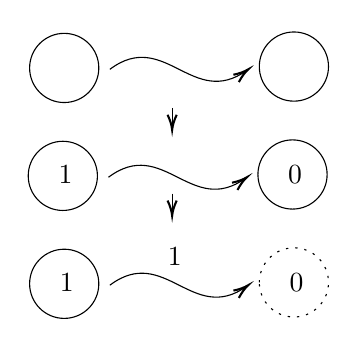
\begin{tikzpicture}[x=0.5pt,y=0.5pt,yscale=-1,xscale=1]
%uncomment if require: \path (0,227); %set diagram left start at 0, and has height of 227

%Shape: Circle [id:dp17666476220496174] 
\draw   (211,33) .. controls (211,19.19) and (222.19,8) .. (236,8) .. controls (249.81,8) and (261,19.19) .. (261,33) .. controls (261,46.81) and (249.81,58) .. (236,58) .. controls (222.19,58) and (211,46.81) .. (211,33) -- cycle ;
%Curve Lines [id:da39834633310900913] 
\draw    (269,34) .. controls (308.6,4.3) and (328.6,62.81) .. (367.81,34.87) ;
\draw [shift={(369,34)}, rotate = 143.13] [color={rgb, 255:red, 0; green, 0; blue, 0 }  ][line width=0.75]    (10.93,-3.29) .. controls (6.95,-1.4) and (3.31,-0.3) .. (0,0) .. controls (3.31,0.3) and (6.95,1.4) .. (10.93,3.29)   ;
%Shape: Circle [id:dp7534299530726538] 
\draw   (377,32) .. controls (377,18.19) and (388.19,7) .. (402,7) .. controls (415.81,7) and (427,18.19) .. (427,32) .. controls (427,45.81) and (415.81,57) .. (402,57) .. controls (388.19,57) and (377,45.81) .. (377,32) -- cycle ;

%Shape: Circle [id:dp7796210885479526] 
\draw   (210,111) .. controls (210,97.19) and (221.19,86) .. (235,86) .. controls (248.81,86) and (260,97.19) .. (260,111) .. controls (260,124.81) and (248.81,136) .. (235,136) .. controls (221.19,136) and (210,124.81) .. (210,111) -- cycle ;
%Curve Lines [id:da1350715866665244] 
\draw    (268,112) .. controls (307.6,82.3) and (327.6,140.81) .. (366.81,112.87) ;
\draw [shift={(368,112)}, rotate = 143.13] [color={rgb, 255:red, 0; green, 0; blue, 0 }  ][line width=0.75]    (10.93,-3.29) .. controls (6.95,-1.4) and (3.31,-0.3) .. (0,0) .. controls (3.31,0.3) and (6.95,1.4) .. (10.93,3.29)   ;
%Shape: Circle [id:dp4166433288053486] 
\draw   (376,110) .. controls (376,96.19) and (387.19,85) .. (401,85) .. controls (414.81,85) and (426,96.19) .. (426,110) .. controls (426,123.81) and (414.81,135) .. (401,135) .. controls (387.19,135) and (376,123.81) .. (376,110) -- cycle ;

%Shape: Circle [id:dp7454657099545818] 
\draw   (211,189) .. controls (211,175.19) and (222.19,164) .. (236,164) .. controls (249.81,164) and (261,175.19) .. (261,189) .. controls (261,202.81) and (249.81,214) .. (236,214) .. controls (222.19,214) and (211,202.81) .. (211,189) -- cycle ;
%Curve Lines [id:da37001677737447913] 
\draw    (269,190) .. controls (308.6,160.3) and (328.6,218.81) .. (367.81,190.87) ;
\draw [shift={(369,190)}, rotate = 143.13] [color={rgb, 255:red, 0; green, 0; blue, 0 }  ][line width=0.75]    (10.93,-3.29) .. controls (6.95,-1.4) and (3.31,-0.3) .. (0,0) .. controls (3.31,0.3) and (6.95,1.4) .. (10.93,3.29)   ;
%Shape: Circle [id:dp5510165008611709] 
\draw  [dash pattern={on 0.84pt off 2.51pt}] (377,188) .. controls (377,174.19) and (388.19,163) .. (402,163) .. controls (415.81,163) and (427,174.19) .. (427,188) .. controls (427,201.81) and (415.81,213) .. (402,213) .. controls (388.19,213) and (377,201.81) .. (377,188) -- cycle ;

%Straight Lines [id:da33968164998086126] 
\draw    (314,61.8) -- (314,75.8) ;
\draw [shift={(314,77.8)}, rotate = 270] [color={rgb, 255:red, 0; green, 0; blue, 0 }  ][line width=0.75]    (10.93,-3.29) .. controls (6.95,-1.4) and (3.31,-0.3) .. (0,0) .. controls (3.31,0.3) and (6.95,1.4) .. (10.93,3.29)   ;
%Straight Lines [id:da020904954319191038] 
\draw    (314,123.8) -- (314,137.8) ;
\draw [shift={(314,139.8)}, rotate = 270] [color={rgb, 255:red, 0; green, 0; blue, 0 }  ][line width=0.75]    (10.93,-3.29) .. controls (6.95,-1.4) and (3.31,-0.3) .. (0,0) .. controls (3.31,0.3) and (6.95,1.4) .. (10.93,3.29)   ;

% Text Node
\draw (230,102) node [anchor=north west][inner sep=0.75pt]   [align=left] {1};
% Text Node
\draw (396,102) node [anchor=north west][inner sep=0.75pt]   [align=left] {0};
% Text Node
\draw (231,180) node [anchor=north west][inner sep=0.75pt]   [align=left] {1};
% Text Node
\draw (397,180) node [anchor=north west][inner sep=0.75pt]   [align=left] {0};
% Text Node
\draw (309,161) node [anchor=north west][inner sep=0.75pt]   [align=left] {1};

\end{tikzpicture}
\caption{Visualization of the selection phase} 

\end{figure}

\begin{figure}
\centering

\tikzset{every picture/.style={line width=0.75pt}} %set default line width to 0.75pt        

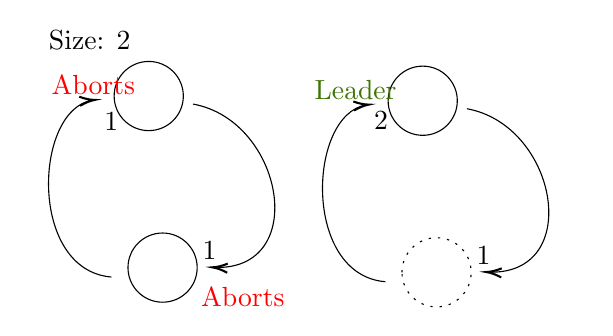
\begin{tikzpicture}[x=0.5pt,y=0.5pt,yscale=-1,xscale=1]
%uncomment if require: \path (0,227); %set diagram left start at 0, and has height of 227

%Shape: Circle [id:dp5018691406521496] 
\draw   (199,65) .. controls (199,51.19) and (210.19,40) .. (224,40) .. controls (237.81,40) and (249,51.19) .. (249,65) .. controls (249,78.81) and (237.81,90) .. (224,90) .. controls (210.19,90) and (199,78.81) .. (199,65) -- cycle ;
%Curve Lines [id:da20396789774914814] 
\draw    (256,70.8) .. controls (321.67,82.74) and (340.81,191.7) .. (271.06,188.85) ;
\draw [shift={(270,188.8)}, rotate = 3.22] [color={rgb, 255:red, 0; green, 0; blue, 0 }  ][line width=0.75]    (10.93,-3.29) .. controls (6.95,-1.4) and (3.31,-0.3) .. (0,0) .. controls (3.31,0.3) and (6.95,1.4) .. (10.93,3.29)   ;
%Shape: Circle [id:dp690252383629637] 
\draw   (209,189) .. controls (209,175.19) and (220.19,164) .. (234,164) .. controls (247.81,164) and (259,175.19) .. (259,189) .. controls (259,202.81) and (247.81,214) .. (234,214) .. controls (220.19,214) and (209,202.81) .. (209,189) -- cycle ;
%Curve Lines [id:da129520635584641] 
\draw    (197,195.8) .. controls (136.91,190.87) and (140.86,75.34) .. (183.05,68.06) ;
\draw [shift={(185,67.8)}, rotate = 174.81] [color={rgb, 255:red, 0; green, 0; blue, 0 }  ][line width=0.75]    (10.93,-3.29) .. controls (6.95,-1.4) and (3.31,-0.3) .. (0,0) .. controls (3.31,0.3) and (6.95,1.4) .. (10.93,3.29)   ;
%Shape: Circle [id:dp564271034205392] 
\draw   (397,68.4) .. controls (397,54.59) and (408.19,43.4) .. (422,43.4) .. controls (435.81,43.4) and (447,54.59) .. (447,68.4) .. controls (447,82.21) and (435.81,93.4) .. (422,93.4) .. controls (408.19,93.4) and (397,82.21) .. (397,68.4) -- cycle ;
%Curve Lines [id:da19396761252410832] 
\draw    (454,74.2) .. controls (519.67,86.14) and (538.81,195.1) .. (469.06,192.25) ;
\draw [shift={(468,192.2)}, rotate = 3.22] [color={rgb, 255:red, 0; green, 0; blue, 0 }  ][line width=0.75]    (10.93,-3.29) .. controls (6.95,-1.4) and (3.31,-0.3) .. (0,0) .. controls (3.31,0.3) and (6.95,1.4) .. (10.93,3.29)   ;
%Shape: Circle [id:dp7609312995918576] 
\draw  [dash pattern={on 0.84pt off 2.51pt}] (407,192.4) .. controls (407,178.59) and (418.19,167.4) .. (432,167.4) .. controls (445.81,167.4) and (457,178.59) .. (457,192.4) .. controls (457,206.21) and (445.81,217.4) .. (432,217.4) .. controls (418.19,217.4) and (407,206.21) .. (407,192.4) -- cycle ;
%Curve Lines [id:da8317353909503531] 
\draw    (395,199.2) .. controls (334.92,194.27) and (338.86,78.74) .. (381.05,71.46) ;
\draw [shift={(383,71.2)}, rotate = 174.81] [color={rgb, 255:red, 0; green, 0; blue, 0 }  ][line width=0.75]    (10.93,-3.29) .. controls (6.95,-1.4) and (3.31,-0.3) .. (0,0) .. controls (3.31,0.3) and (6.95,1.4) .. (10.93,3.29)   ;

% Text Node
\draw (152,48) node [anchor=north west][inner sep=0.75pt]   [align=left] {\textcolor[rgb]{1,0,0}{Aborts}};
% Text Node
\draw (260,201) node [anchor=north west][inner sep=0.75pt]   [align=left] {\textcolor[rgb]{1,0,0}{Aborts}};
% Text Node
\draw (342,52) node [anchor=north west][inner sep=0.75pt]   [align=left] {\textcolor[rgb]{0.25,0.46,0.02}{Leader}};
% Text Node
\draw (190,75) node [anchor=north west][inner sep=0.75pt]   [align=left] {1};
% Text Node
\draw (261,168) node [anchor=north west][inner sep=0.75pt]   [align=left] {1};
% Text Node
\draw (459,172) node [anchor=north west][inner sep=0.75pt]   [align=left] {1};
% Text Node
\draw (385,74.2) node [anchor=north west][inner sep=0.75pt]   [align=left] {2};
% Text Node
\draw (150,16) node [anchor=north west][inner sep=0.75pt]   [align=left] {Size: 2};


\end{tikzpicture}
\caption{Visualization of the verification phase}
\end{figure}

\subsection{Implementation}
An implementation of the algorithm is pretty straightforward and convenient due to the fact that the process know how many messages should receive and send in the selection phase. The processes communicate between each other by well structured and lightweight messages. They also have their own states used in order to recognise their function. Since the algorithm is randomised, it can fail sometimes, but the reinvocation is implemented.
\subsubsection{Message structure}
Messages structure is implemented as follows:
\begin{itemize}
    \item \textsc{MessageType} 
    \item \textsc{Data} (\texttt{[]byte})
\end{itemize}

Where \textsc{MessageType} can be one of the following:
\begin{itemize}
    \item Elimination -- message in the selection phase of the algorithm
    \item Counter -- message in the verification phase of the algorithm 
    \item Elected -- just to confirm that the leader is elected, used to stop 
\end{itemize}

\subsubsection{Process state}
Each process has one of the following states.
\begin{itemize}
    \item Unknown -- the process is active, but not yet leader
    \item Nonleader -- the process is inactive
    \item Leader -- the process is a leader
\end{itemize}
Initially every process has \textit{Unknown} state
\section{Correctness and complexity analysis}
    A leader election algorithm may return incorrect answer in two cases: if it elected more than one leader or no process were elected. However, in our algorithm the following happen:
    \begin{itemize}
        \item It is highly likely that after $c=5\log n$ rounds of selection phase there will be no more than one active process. In case of the bad luck, we can just reinvoke it.
        \item Always at least one process is active; If any process becomes inactive, then it must be at least one which got bit 1.
    \end{itemize}


\subsection{Bit complexity analysis}
    We assume that we flip fair coin here (1 and 0 with prob. $\frac{1}{2}$). The probability that an active process becomes inactive in a round is $\frac{1}{4}$. Therefore, by linearity of expectations, expected number of processes which become inactive in round 1 is $\frac{n}{4}$ . So the expected number of rounds until only one process remains active is $\log_{4/3}{n}$. If we choose $c>2\log_{4/3}{n} \approx 4.8188 \log {n}$ then the probability that more than one process remains active after $c$ rounds is small\cite{itairodeh}. The total bit complexity of the selection phase is $cn=\mathcal{O}(n\log n)$. In the verification phase it is $a\mathcal{O}(n \log n )$, where $a=1$ is expected number of active processes after $c$ rounds.

\subsection{Probabilistic analysis}
Let $X_t$ - number of active processes which became inactive in stage $t$
\\Also $$D_t = \sum_{i=1}^t X_i$$ $$N_t = n-D_t$$ $$Q_t(z)=\sum_{d\geq 0} \Pr(D_t = d)z^d$$
We can calculate probability of $X_1 = k$
    $$\Pr(X_1 = k)=2^{-n+1}\binom{n}{2k}$$
    $$Q_1(z) = \sum_{k\geq 0} \Pr(X_1 = k) z^k = 2^{-n}[(1+\sqrt{z})^n + (z-\sqrt{z})^n]$$
    $$E(X_1) = Q_1'(1) = \frac{n}{4}$$
    $$E(X_1^2) = Q_1''(1) + E(X_1) = \frac{n(n+1)}{16}$$
We define $\tilde{N}$ such that $$E(\tilde{X} | \tilde{D}_{t-1}=d)=\frac{n-d}{4}$$
Thus $$N_t=
\begin{cases}
		    N_t, & {N_t > 1}\\
            1, & \text{otherwise}
\end{cases}$$
\begin{lemma}
$$E(\tilde{D}_t) = n(1-(3/4)^t)$$
\\$$V(\tilde{D}_t) = \frac{n}{3} \Bigm[\Bigm(\frac{3}{4}\Bigm)^t - \Bigm(\frac{3}{4}\Bigm)^{2t}\Bigm]$$
\end{lemma}

\begin{lemma}
$$\Pr(N_t > 1) \leq (n/3)(3/4)^t + n((3n-1)/3)(3/4)^{2t}$$
\end{lemma}
\begin{proof}

By Chebychev's inequality
$$\Pr(N_t > 1) \leq E(N_t^2) = E((n-\tilde{D}_t)^2) = \frac{n}{3}\Bigm(\frac{3}{4}\Bigm)^t + n \frac{3n-1}{3}\Bigm(\frac{3}{4}\Bigm)^{2t}$$
\end{proof}
\begin{corollary}
For $c(n)/\log n > 2/\log_2 {4/3} \approx 4.8188417 $ the expected communication complexity of the algorithm is $\mathcal{O}(n \log n)$ bits
\end{corollary}

\printbibliography
\end{document}
